\documentclass[12pt]{article}
\usepackage[utf8]{inputenc}
\usepackage{enumitem}
\usepackage{scalefnt}
\usepackage{graphicx}
\usepackage{afterpage}
\usepackage{tikz-uml}
\usepackage[english]{babel}
\usepackage{fullpage}
\usepackage{float}
\usepackage{amsmath}
\usepackage[T1]{fontenc}
\usepackage{xcolor}
\usepackage[colorlinks=true,linkcolor=green]{hyperref}
% \usepackage{layaureo}


% \usepackage{fancyhdr}
\usepackage{geometry}
\geometry{
  paper=a4paper,
  inner=3cm,
  outer=3cm,
  top=3cm,
  bottom=3cm,
  footskip=.5cm
}
% \usepackage{ragged2e}
% \RaggedRight
\usepackage[none]{hyphenat}

\begin{document}

\large

\newpage

\date{}

\vspace*{10pt}
\begin{center}
{\Huge Database Management Systems} \\[40pt]
{\LARGE Software Requirements Specification} \\[15pt]
\textit{\large for} \\[15pt]
\textbf{\LARGE Sports Slot Booking System (SSBS)} \\[15pt]
\textit{\large submitted by} \\[25pt]
\end{center}
\hspace{2.2cm}{\Large Vignesh Aravindh B} \hspace{1cm} \textbf{\Large CS22B2004} \\[10pt]
\hspace*{2.2cm}{\Large Rajvardhan G} \hspace{2.505cm} \textbf{\Large CS22B2013} \\[10pt]
\hspace*{2.2cm}{\Large Ashrith G} \hspace{3.53cm} \textbf{\Large CS22B2025} \\[10pt]
\hspace*{2.2cm}{\Large P Veeresh Kumar} \hspace{1.725cm} \textbf{\Large CS22B2026} \\[10pt]
\hspace*{2.2cm}{\Large Dhivya Dharshan V} \hspace{1.185cm} \textbf{\Large CS22B2053}

\newpage

\tableofcontents
\listoffigures

\newpage

\section{Introduction}
\hspace{0.8cm} The \textbf{Sports Slot Booking System (SSBS)} is an \textit{online platform} designed to facilitate the reservation of sports slots for institute students, allowing them to `book slots' for their regular indoor sports activities throughout the semester. This System Requirements Specification (SRS) outlines the `essential functionalities', `system requirements' and `operational constraints' of SSBS, providing a clear framework for its development and integration within the institute's ``infrastructure".

\vspace{0.4cm}

\section{Purpose}
\hspace{0.8cm} The purpose of \textbf{SSBS} is to make booking slots for indoor sports activities like \textit{Badminton, Carrom, Chess, Gym and Table Tennis} easier with an `online platform'. It aims to ensure that users can `book their preferred slots' conveniently, maximizing the use of sports facilities. SSBS strives to `simplify the booking process', `reduce scheduling conflicts' and enhance the overall experience of users engaging in indoor sports. By providing a ``straightforward and user-friendly solution", SSBS aims to promote active participation in sports activities and contribute to the well-being of the ``IIITDM community".

\vspace*{0.4cm}

\section{Scope}
\hspace{0.8cm} The scope of \textbf{SSBS} encompasses various key components essential for efficient sports facility management. It will cover aspects such as `managing different sports activities', `defining available slots', `tracking slot availability' and facilitating slot bookings for \textit{students, faculty and staff members}. Additionally, SSBS will provide functionalities for `maintaining user accounts', `handling booking requests', `generating reports on sports facility utilization' and ensuring users and administrators can ``communicate smoothly".

\vspace{0.4cm}

\section{Functional Requirements for Sports Slot Booking System (SSBS)}

\begin{enumerate}
    
    \item[] \subsection{User Authentication and Profile Management:}
    \begin{enumerate}[label=\alph*)]
        \item Implement authentication mechanism using institute-provided email IDs for \textit{students, faculty and staff members}.
        \item `Verify user identity' by cross-referencing entered ID with the respective tables from the database for students, faculty and staff members.
        \item Allow users to `update contact details' such as phone number.
        \item `Ensure data integrity' by validating user inputs, to prevent unauthorized access or tampering.
    \end{enumerate}

    \vspace{0.4cm}

    \item[] \subsection{Sports Management:}
    \begin{enumerate}[label=\alph*)]
        \item `Define and maintain a list' of available sports activities.
        \item Specify `maximum capacity' and other relevant details for each sport activity.
        \item Provide an intuitive interface for administrators to `add, edit or remove sports activities' as required.
    \end{enumerate}

    \vspace{0.4cm}

    \item[] \subsection{Slot Booking:}
    \begin{enumerate}[label=\alph*)]
        \item Display a `unified interface' for booking slots across all available sports activities.
        \item Allow users to select their `desired sport and available slot'.
        \item Restrict users to booking only `one slot per sport activity, at a time'.
        \item Implement `real-time validation' to prevent double booking and ensure slot availability.
        \item Provide `confirmation messages' upon successful booking and display booked slots in user profiles.
    \end{enumerate}

    % \vspace{0.5cm}
    \newpage

    \item[] \subsection{Dependency Management:}
    \begin{enumerate}[label=\alph*)]
        \item Enable faculty members to `register their dependents' using their institute-provided email IDs.
        \item `Associate each dependent' with the respective faculty member upon registration.
        \item Implement checks to ensure that `dependents are not registered under multiple faculty members' simultaneously.
    \end{enumerate}

    \vspace{0.4cm}

    \item[] \subsection{Registration Period Management:}
    \begin{enumerate}[label=\alph*)]
        \item `Record registration start and end dates' for each user account.
        \item Define end dates based on specific time intervals such as `one semester, month or week'.
        \item `Notify users' about upcoming registration periods and expiration dates of their subscriptions.
        \item Upon the expiration of a subscription period, individuals who previously subscribed to a particular slot will no longer have access to that slot unless they renew their subscription by booking again. This ensures that access to slots is regulated according to ``active subscriptions", promoting fairness and efficient utilization of sports facilities.
    \end{enumerate}

    \vspace{0.4cm}

    \item[] \subsection{Reporting and Analytics:}
    \begin{enumerate}[label=\alph*)]
        \item `Generate reports' about users, sports facility utilization and booking trends.
        \item Provide insights into `popular sports activities', `peak booking times' and `user participation rates'.
        \item Allow administrators to export reports in various formats for analysis and decision-making purposes.
    \end{enumerate}
   
\end{enumerate}

\vspace{0.2cm}

\newpage

\noindent These functional requirements are tailored to ensure smooth operation of the \textbf{Sports Slot Booking System (SSBS)}, with a focus on `user authentication', `profile management' and `efficient booking processes' while adhering to the unique requirements of the ``IIITDM community".

\section{Non-Functional Requirements}

\begin{enumerate}[label=\arabic*.]
    \item[] \subsection{Performance:}
    \begin{enumerate}[label=\alph*)]
        \item `Ensure the system can handle concurrent user access and booking requests' without performance degradation.
        \item `Response times' for slot availability and booking operations should be within acceptable limits.
    \end{enumerate}

    \vspace{0.4cm}

    \item[] \subsection{Scalability:}
    \begin{enumerate}[label=\alph*)]
        \item Design the system to `accommodate increasing numbers of users and booking requests' over time.
        \item Ensure `scalability of database' to manage large volumes of user data and booking records.
    \end{enumerate}

    \vspace{0.4cm}

    \item[] \subsection{Security:}
    \begin{enumerate}[label=\alph*)]
        \item Implement `authentication mechanisms' to verify user identities during login.
        \item `Encrypt sensitive user data' such as personal information to maintain confidentiality.
        \item Apply `access controls' to restrict unauthorized access to booking functionalities.
    \end{enumerate}

    \vspace{0.4cm}

    \newpage
    
    \item[] \subsection{Usability:}
    \begin{enumerate}[label=\alph*)]
        \item Design an `intuitive user interface' with clear navigation and booking instructions.
        \item Get `informative feedback messages' to enhance user experience.
    \end{enumerate}
   
\end{enumerate}



\section{Constraints}
\hspace{0.8cm} The \textbf{Sports Slot Booking System (SSBS)} must use `technology and platforms' that work with the organization's existing setup. It also needs to follow the `rules and standards for developing and testing software' that are important in our field.

\vspace{0.4cm}

\section{Conclusion}
\hspace{0.8cm} The \textbf{Sports Slot Booking System (SSBS)} aims to improve the reservation process for indoor sports activities at IIITDM. By providing a `user-friendly platform' for booking sports slots, SSBS promotes `active participation' and `effective utilization of sports facilities'. With a focus on ``performance, scalability, security, and usability", SSBS will help create a healthier and livelier sports community at the ``institute".

\newpage

\begin{itemize}
    \begin{figure}[h]
    \centering
    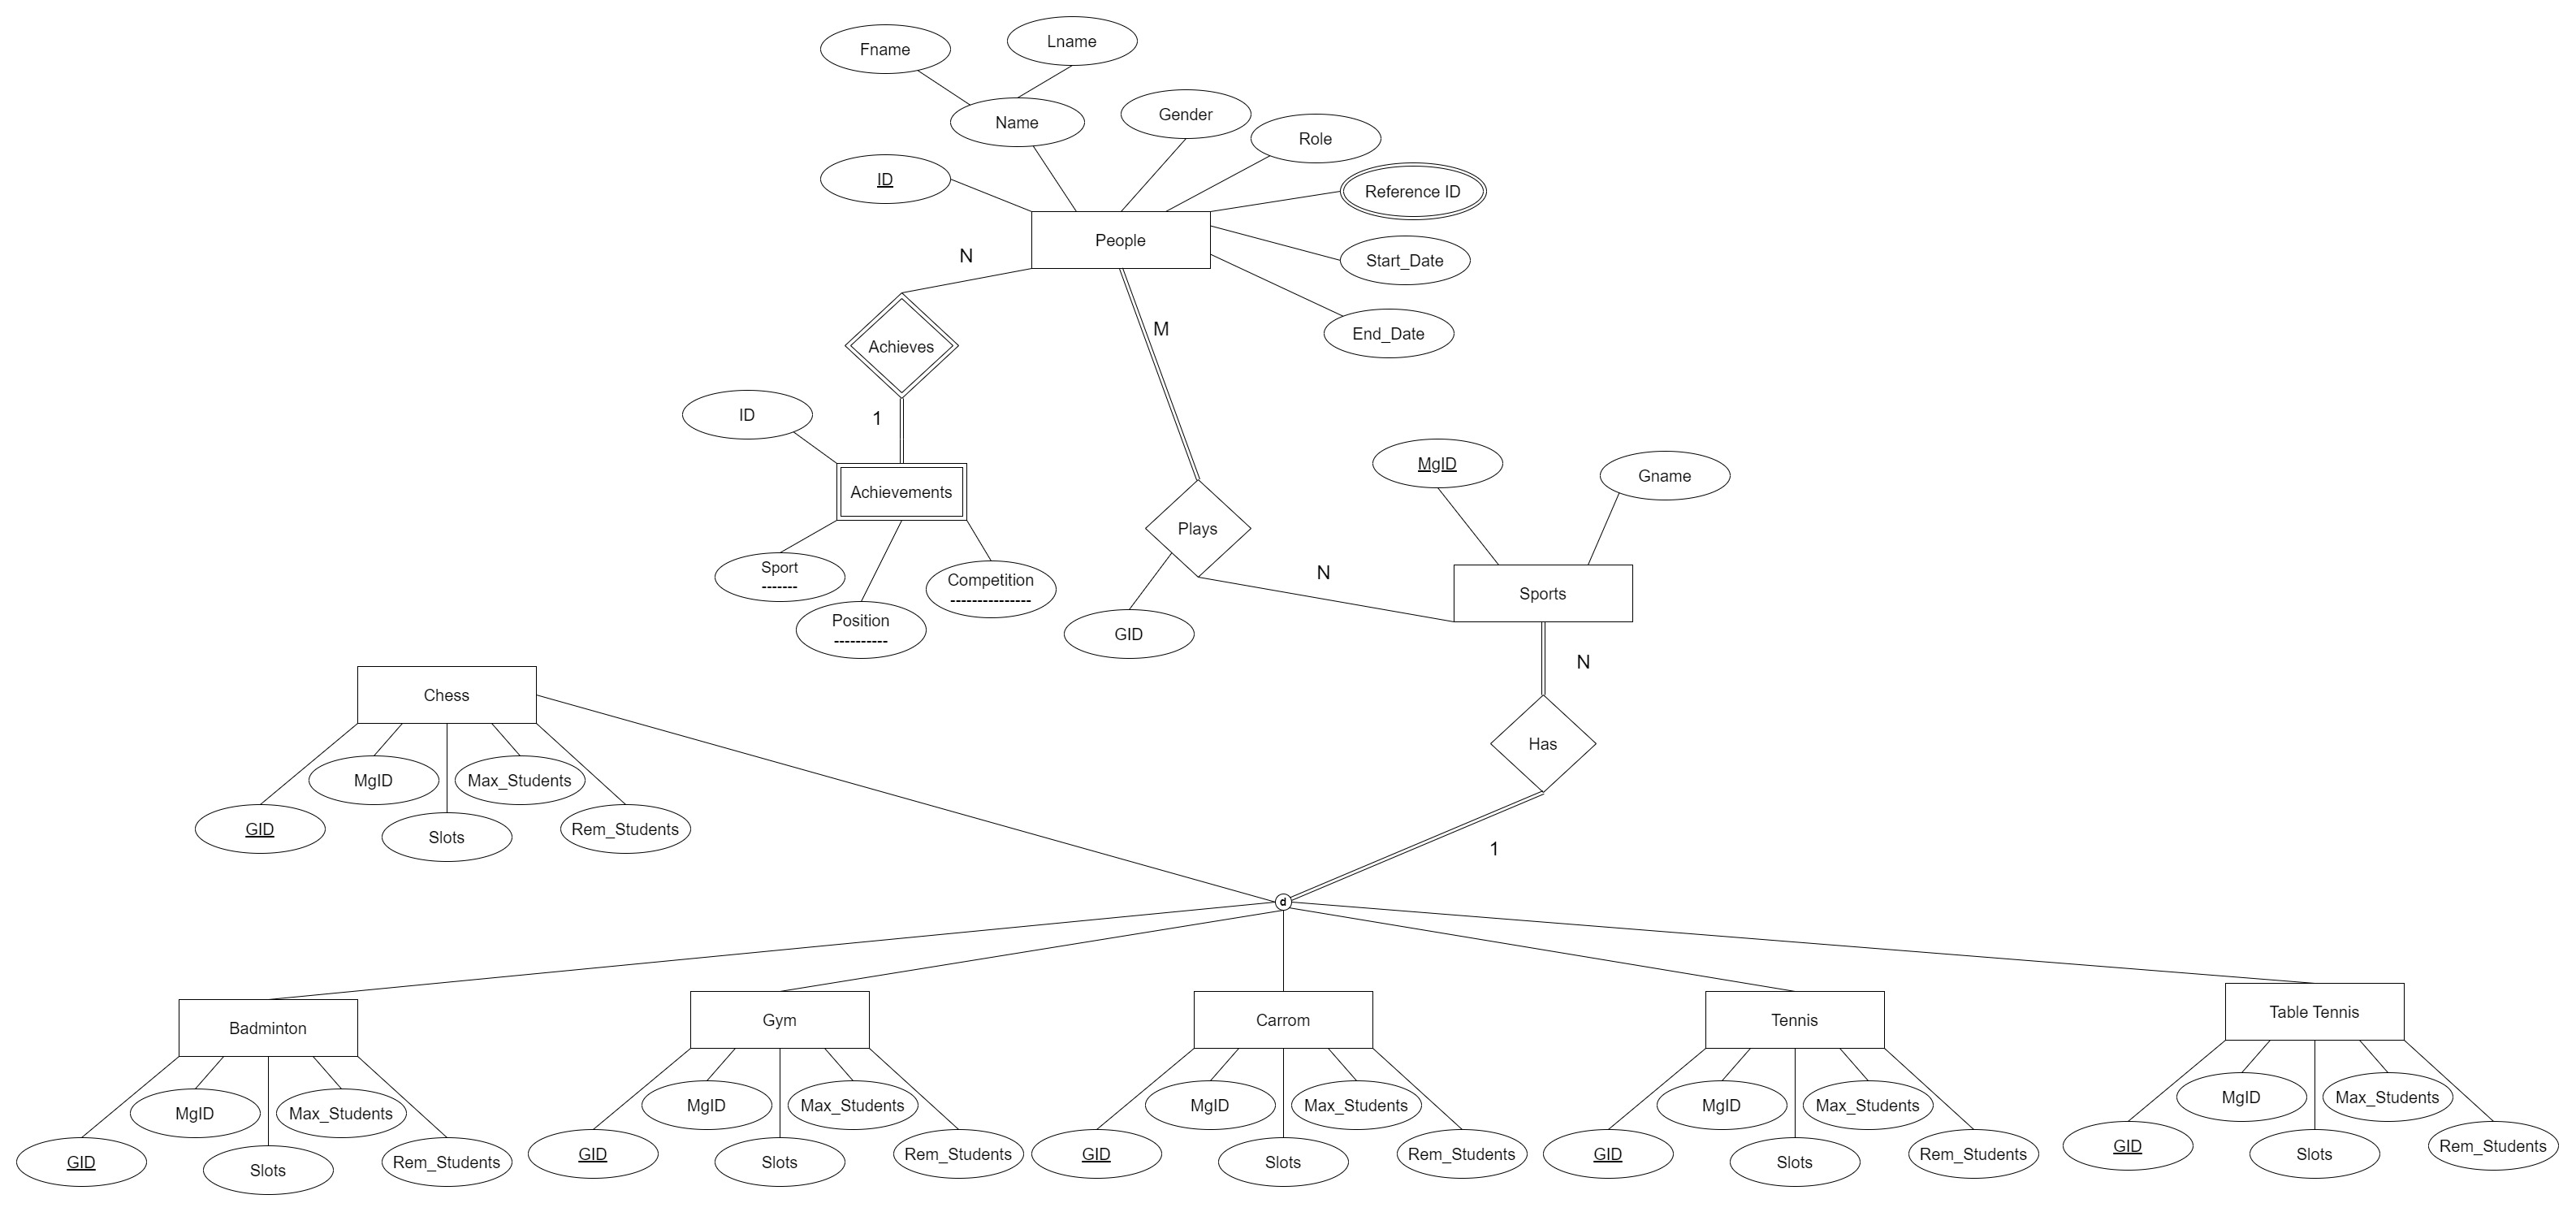
\includegraphics[width=1\linewidth]{ER4.jpg}
    \caption{ER diagram}
    \label{fig:enter-label}
    \end{figure}
\end{itemize}

\newpage
\afterpage{%
\begin{figure}[H] % Use H specifier to force the figure to appear "Here"
\centering
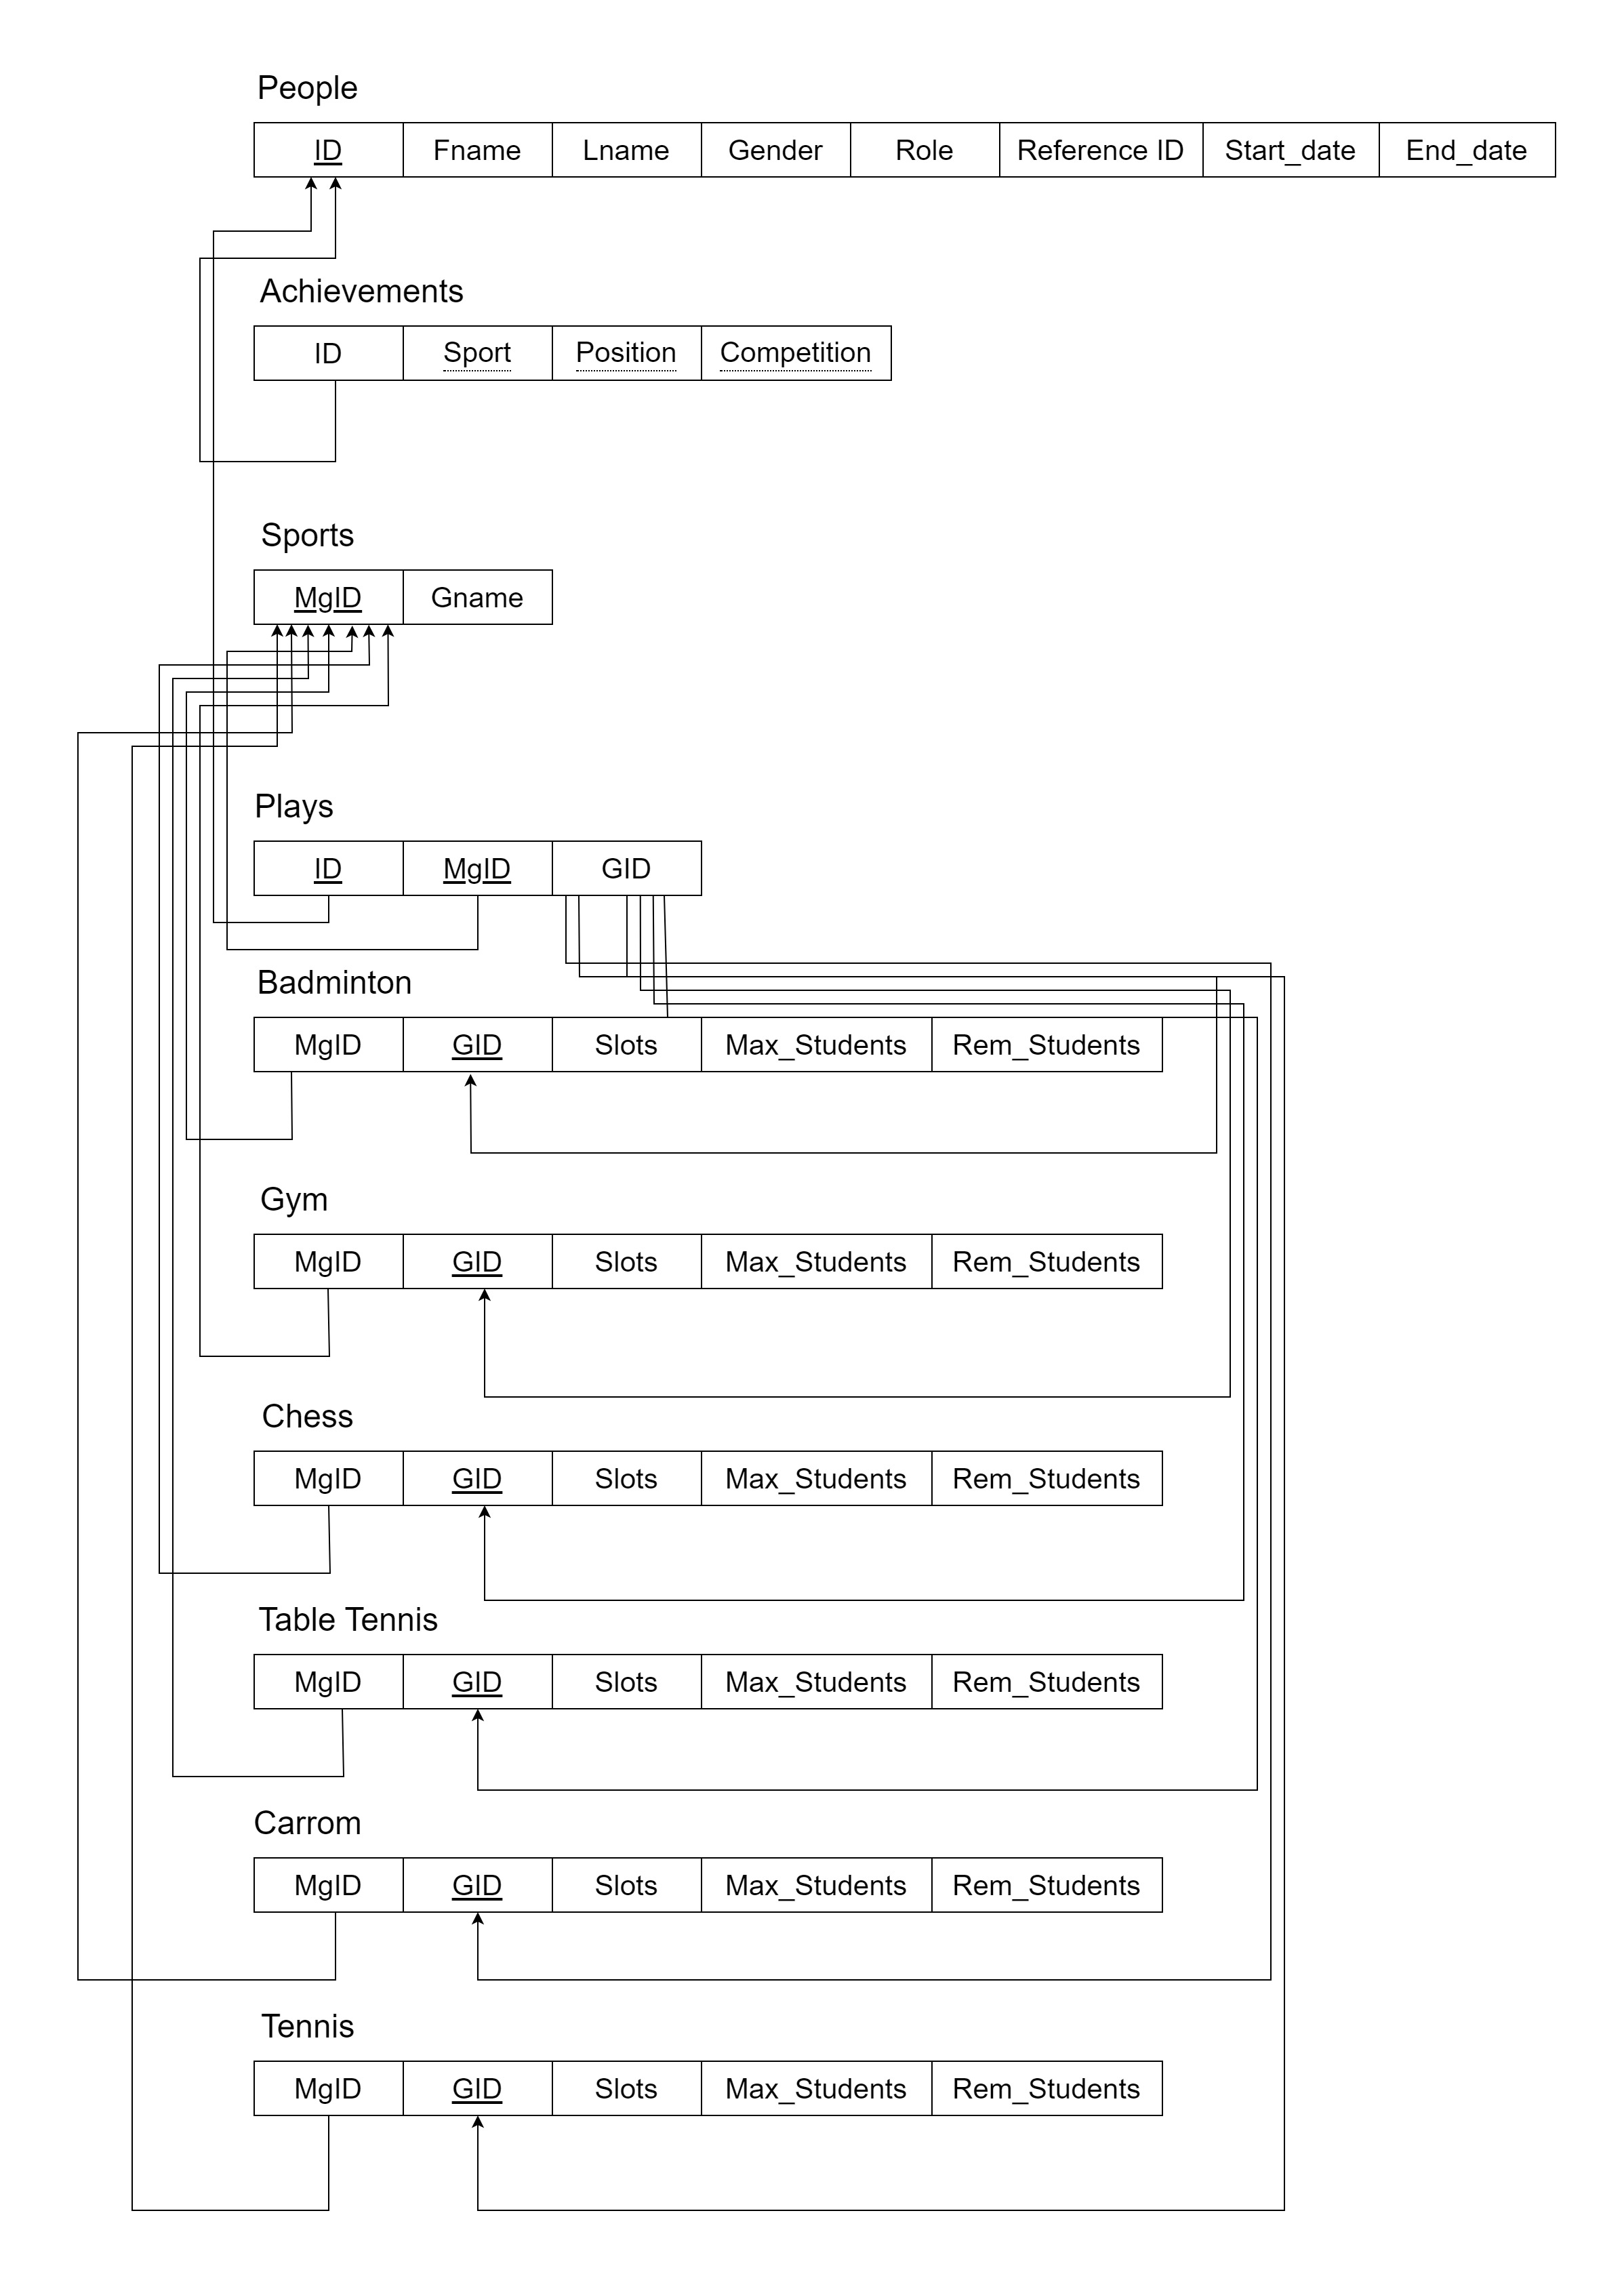
\includegraphics[width=1\linewidth]{schema1.jpg}
\caption{Schema Diagram}
\label{fig:enter-label}
\end{figure}
}

%
% Compilation of the examples from the TikZ-UML manual, v. 1.0b (2013-03-01)
% http://www.ensta-paristech.fr/~kielbasi/tikzuml/index.php?lang=en
%

% \usepackage{layaureo}
\newpage
\afterpage{

\begin{figure}[H]
    \centering
    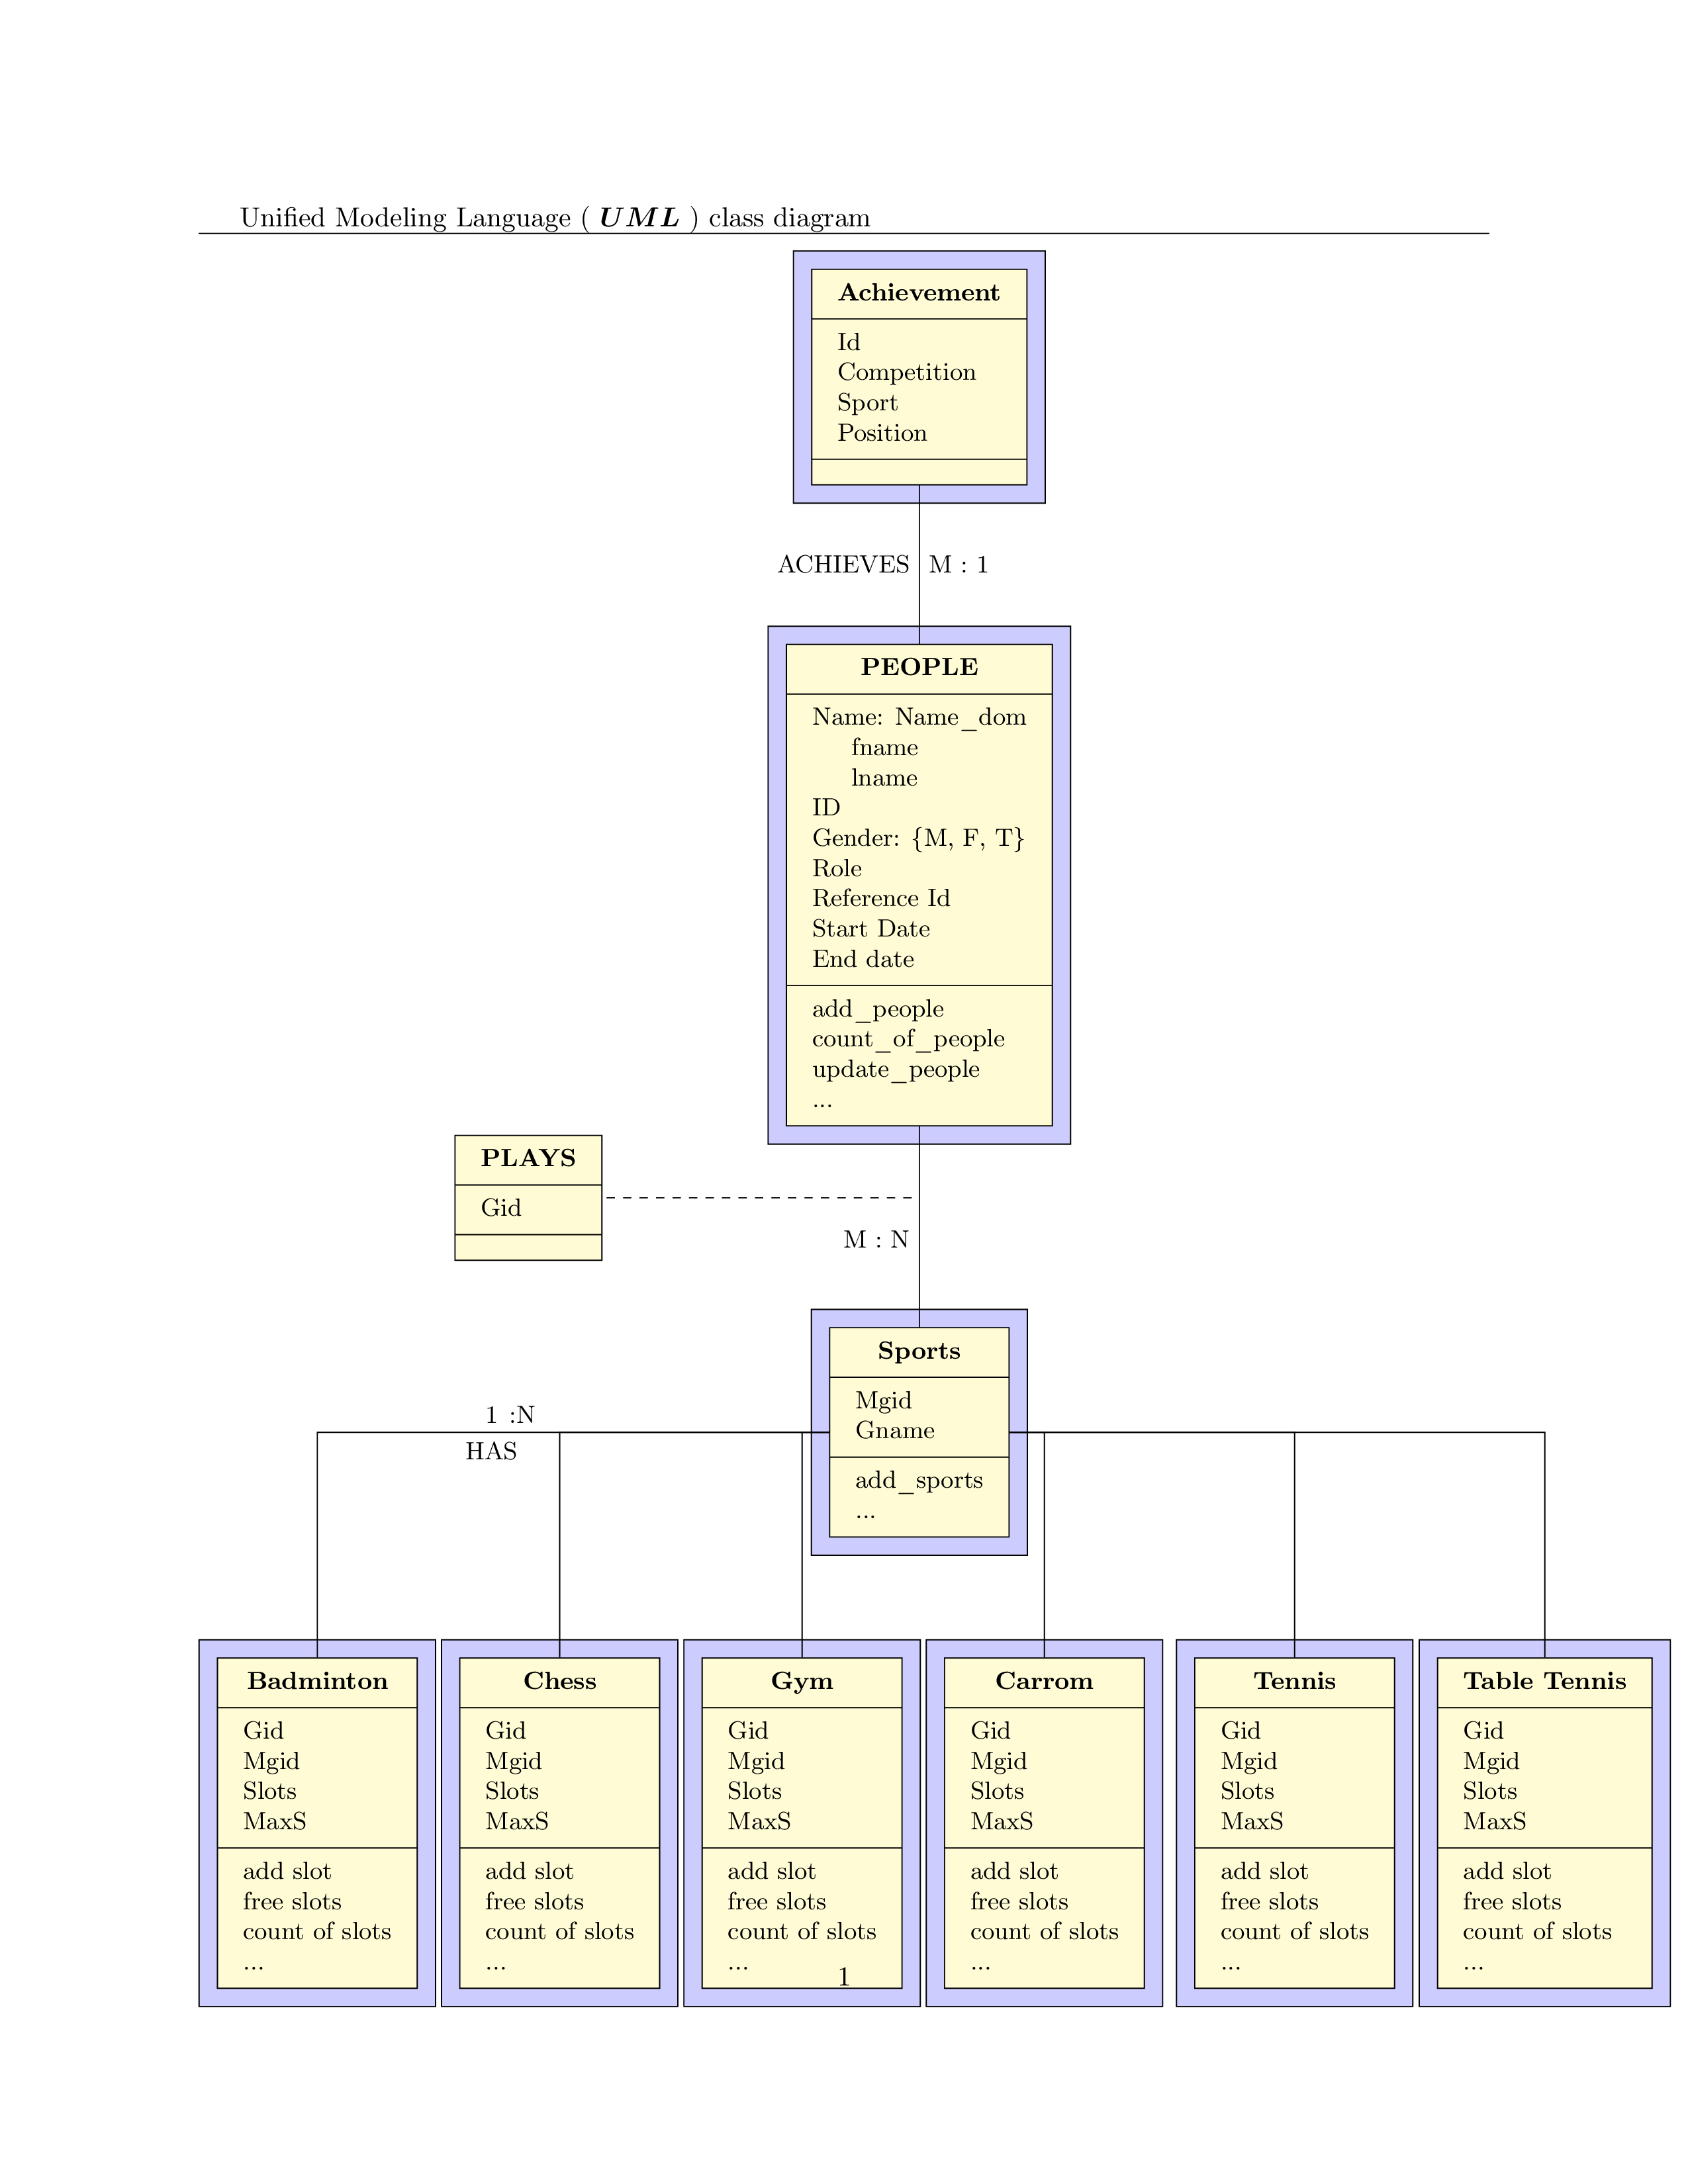
\includegraphics[width=\linewidth]{uml_diagram.png}
    \caption{Unified Modeling Language (UML) class diagram}
    \label{fig:uml-diagram}
\end{figure}
}

\clearpage
\newpage

\noindent \Large Link for the SRS code files: 
\begin{center}
    \href{https://github.com/RajV95/DBMS}{https://github.com/RajV95/DBMS}
\end{center}

\begin{center}    
    \Huge Thank You!    
\end{center}
    
\end{document}


\end{document}
\textit{\textit{}}

